\documentclass[italian,a4paper]{article}
\usepackage[tight,nice]{units}
\usepackage{babel,amsmath,amssymb,amsthm,graphicx,url}
\usepackage[text={5.5in,9in},centering]{geometry}
\usepackage[utf8x]{inputenc}
\usepackage[T1]{fontenc}
\usepackage{ae,aecompl}
\usepackage[footnotesize,bf]{caption}
\usepackage[usenames]{color}
\usepackage{textcomp}
\usepackage{gensymb}
%\include{pstricks}
\frenchspacing
\pagestyle{plain}
%------------- eliminare prime e ultime linee isolate
\clubpenalty=9999%
\widowpenalty=9999
%--- definizione numerazioni
\renewcommand{\theequation}{\thesection.\arabic{equation}}
\renewcommand{\thefigure}{\arabic{figure}}
\renewcommand{\thetable}{\arabic{table}}
\addto\captionsitalian{%
  \renewcommand{\figurename}%
{Grafico}%
}
%
%------------- ridefinizione simbolo per elenchi puntati: en dash
%\renewcommand{\labelitemi}{\textbf{--}}
\renewcommand{\labelenumi}{\textbf{\arabic{enumi}.}}
\setlength{\abovecaptionskip}{\baselineskip}   % 0.5cm as an example
\setlength{\floatsep}{2\baselineskip}
\setlength{\belowcaptionskip}{\baselineskip}   % 0.5cm as an example
%--------- comandi insiemi numeri complessi, naturali, reali e altre abbreviazioni
\renewcommand{\leq}{\leqslant}
%--------- porzione dedicata ai float in una pagina:
\renewcommand{\textfraction}{0.05}
\renewcommand{\topfraction}{0.95}
\renewcommand{\bottomfraction}{0.95}
\renewcommand{\floatpagefraction}{0.35}
\setcounter{totalnumber}{5}
%---------
%


%---------
\begin{document}
\title{Relazione di laboratorio: il prisma}
\author{\normalsize Ilaria Brivio (582116)\\%
\normalsize \url{brivio.ilaria@tiscali.it}%
\and %
\normalsize Matteo Abis (584206)\\ %
\normalsize \url{webmaster@latinblog.org}}
\date{\today}
\maketitle
%------------------
\section{Obiettivo dell'esperienza}
L'obiettivo dell'esperienza è la stima dell'indice di rifrazione di un prisma per cinque diverse lunghezze d'onda dello spettro di emissione di una lampada al cadmio e la verifica della formula di Cauchy, che lega queste due grandezze.
\section{Descrizione dell'apparato strumentale}
L'apparato è costituito da un prisma di vetro Crown (K) a base triangolare, fissato a una base che può ruotare attorno ad un asse fisso, e da un cannocchiale per l'osservazione dei raggi luminosi vincolato allo stesso asse. I due elementi possono essere spostati con precisione grazie ad apposite chiavi micrometriche e l'angolo tra le  posizioni dei loro sostegni è misurato con due nonii, $A$ e $B$, di sensibilità 2'. Le scale graduate dei due nonii sono incise sulle stesse giere metalliche e diametralmente opposte l'una all'altra, allo scopo di eliminare l'errore di eccentricità. Inoltre, l'immagine prodotta dal cannocchiale può essere ottimizzata agendo su un diaframma posto davanti alla sorgente e sulle lenti dello strumento stesso.


Sul prisma incide un fascio di luce proveniente da una lampada al cadmio, che emette radiazioni visibili di colore rosso, verde, blu scuro (che chiameremo blu 1), blu chiaro (blu 2) e violetto. 
\section{Descrizione della metodologia di misura}
\subsection*{Misura dell'angolo $\alpha$ tra due facce del prisma}
Dopo aver scelto le due facce di incidenza ed emergenza della luce dal prisma, è stato misurato con precisione l'angolo di apertura $\alpha$ tra di esse, sfruttando il fenomeno della riflessione.

Una volta fissato il cannocchiale nella sua posizione di fine corsa, a formare un angolo acuto con la direzione di incidenza della luce, è stato ruotata la piattaforma del prisma fino a vedere al centro dell'oculare il raggio riflesso sulla prima delle due facce. Sono state registrate le misure riportate da cisacuno dei due nonii in questa configurazione e l'operazione è stata quindi ripetuta per l'altra faccia del prisma.

La deviazione angolare $\Delta \theta$ tra le due configurazioni è pari a $\Delta\theta=\pi-\alpha$, da cui, mediando sulle misure dei due nonii, si è ottenuto $\alpha=$ 60 \textdegree 2.75'.
\subsection*{Misura dell'angolo $\delta$ di deviazione minima}
In generale, la relazione che lega gli angoli di incidenza dei raggi entrante e uscente con l'angolo di deviazione è piuttosto complessa. Risulta però notevolmente sempificata nei due casi di emergenza normale (raggio uscente perpendicolare alla faccia corrispondente del prisma) e di minima deviazione dei raggi. Durante l'esperienza si è operato in una configurazione del secondo tipo.

Innanzitutto sono stati posizionati prisma e cannocchiale in modo da far incidere ed emergere la luce dalle due facce scelte in precedenza e da vedere distintamente il fascio rifratto. A questo punto sono state ruotate nello stesso verso, avvicinandosi alla direzione del fascio incidente, sia la piattaforma del cannocchiale che quella del prisma: la posizione in cui si osserva che la banda di un dato colore inverte il proprio senso di spostamento corrisponde proprio alla minima deviazione per quella lunghezza d'onda. L'angolo $\delta_{\min}$ è quello compreso tra questa posizione del cannocchiale e la direzione di incidenza del fascio. Per fornirne una stima è stata calcolata la differenza tra i valori riportati da ciascun nonio quando il cannocchiale è allineato col raggio rifratto e col raggio indeflesso; si è assunto poi come valore per $\delta_{\min}$ la media aritmetica delle misure dei due nonii.

Seguendo questo procedimento sono stati misurati gli angoli di minima deviazione per ciascuna delle cinque lunghezza d'onda visibili.
\section{Risultati sperimentali ed elaborazione dati}
Nelle condizioni di minima deviazione gli angoli di incidenza dei raggi entrante e uscente dal prisma sono uguali tra loro e per ciascuna lunghezza d'onda $\lambda$, detto $n(\lambda)$ l'indice di rifrazione corrispondente, vale la relazione:
\begin{equation*}
n(\lambda)\sin\dfrac{\alpha}{2}=\sin\dfrac{\alpha+\delta_{\min}(\lambda)}{2}
\end{equation*}
da cui è stato possibile ricavare i valori di $n(\lambda)$, che sono riportati nella tabella seguente, assieme alle lunghezze d'onda corrispondenti. Gli errori su $n$ sono stati calcolati sommando in quadratura e considerando come errore su $\delta_{\min}$ un errore di 2', calcolato a posteriori con un test del chi quadro.
\begin{table}[!h]
\centering
\renewcommand{\arraystretch}{1.2}
\begin{tabular}{ccr@{ $\pm$ }l}
Colore&		$\lambda$ (\unit{nm})&	\multicolumn{2}{c}{$n$}\\\hline
rosso&		643.8&			1.51179 &0.00038 \\
verde&		508.6&			1.51856 &0.00037 \\
blu 2&		480.0&			1.52080 &0.00034 \\
blu 1&		467.8&			1.52118 &0.00037 \\
violetto&	398.2&			1.52398 &0.00037
\end{tabular}
\end{table}\\
La formula di Cauchy fornisce la relazione esplicita tra $n$ e $\lambda$:
\begin{equation*}
n(\lambda)=A+\dfrac{B}{\lambda^2}
\end{equation*}
dove $A$ e $B$ sono parametri caratteristici del materiale con cui è realizzato il prisma di cui vogliamo fornire una stima.
Pertanto è stato realizzato un grafico con lunghezze d'onda in ascissa e indici di rifrazione in ordinata ed è stato eseguito un fit con una curva del tipo $y=a+b/x^2$ (Grafico \ref{cauchy}). Dal fit è stato però escluso il punto corrispondente al violetto, la cui lunghezza d'onda si trova al di fuori dell'intervallo di validità della legge di Cauchy, e che risulta infatti lontano dalla curva teorica.

Dall'interpolazione si è trovato:
\begin{eqnarray*}
A = 1.50106 \pm 0.00087&
B = \unit[4484 \pm 224]{nm^2}
\end{eqnarray*}
con coefficiente di correlazione tra i parametri $r=0.97667$.

Infine, per valutare la bontà della funzione di Cauchy sui dati misurati, è stato calcolato il parametro
\begin{equation}
t=r\sqrt{\dfrac{n-2}{1-r^2}} = 6.431
\end{equation}
dove $n=4$ è il numero di punti e $r$ il coefficiente di correlazione tra i parametri del fit, come riportato sopra. Sapendo che tale parametro è distribuito come la $t$ di Student a $n-2$ gradi di libertà, possiamo così stimare la probabilità $p$ che l'ipotesi zero assunta, ovvero che $\lambda$ e $n$ siano distribuiti secondo la funzione di Cauchy, sia errata.

Tale probabilità è dunque pari all'integrale della funzione densità di probabilità della distribuzione di Student per la variabile $t$ e nel nostro caso risulta $p = 1.17 \%$, dunque possiamo concludere che la legge può essere ritenuta valida con una confidenza del $98.83\%$.
% \section{Conclusioni}


\newpage
\section{Appendice}
% \subsection*{Grafici}
\begin{figure}[!h]\centering
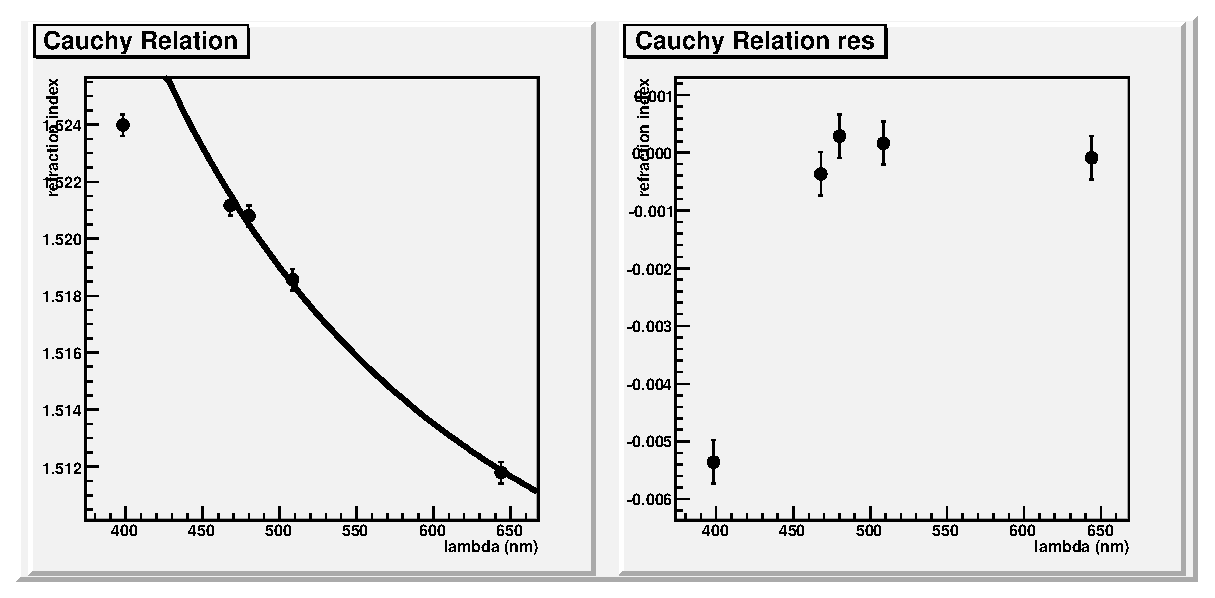
\includegraphics[scale=.6]{cauchy.eps}
\caption{Grafico con lunghezze d'onda (\unit{nm}) in ascissa e indici di rifrazione in ordinata. \`{E} stato eseguito un fit cona una curva del tipo $y=a+b/x^2$ per verificare la legge di Cauchy. Nel grafico a destra sono riportati i residui dell'interpolazione. \`{E} evidente che per il punto corrispondente alla luce violetta la legge non è valida; per questo motivo tale punto è stato escluso dal fit.}\label{cauchy}
\end{figure}
\end{document}
